   
\documentclass[11pt]{article}
\renewcommand{\baselinestretch}{1.05}
\usepackage{amssymb, amsmath, amsfonts, multirow, graphicx}
\topmargin0.0cm
\headheight0.0cm
\headsep0.0cm
\oddsidemargin0.0cm
\textheight23.0cm
\textwidth16.5cm
\footskip1.0cm

\begin{document}

\title{CISC 2210 Discrete Structures - Noson S. Yanofsky}
\author{Student: Ruslan Pantaev}
\maketitle

\section*{1.7}
%
%
\subsection*{1.}
\begin{center}
Let $S = \{1,2,3,4,5\} \text{ and } T = \{a,b,c,d\}$. For each question below: if the answer is Yes, give an example, else explain briefly.\\
\begin{figure}[h!]
	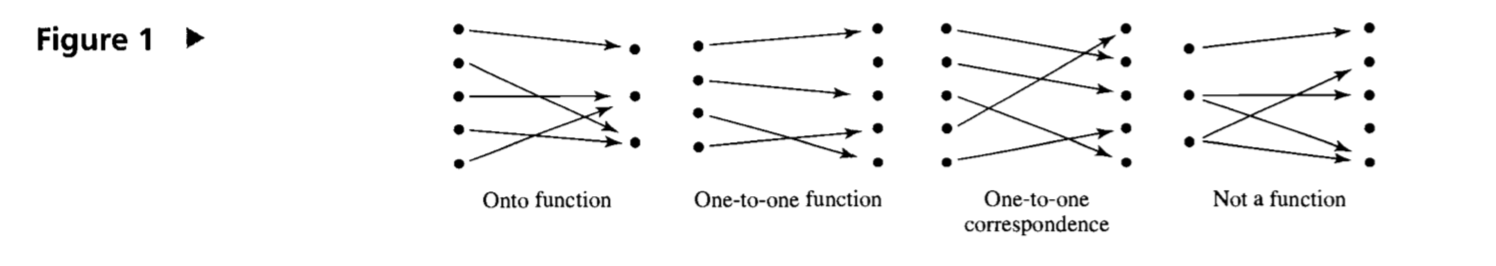
\includegraphics[width=\linewidth]{figure1_types_of_functions.png}
	\caption{types of functions}
	\label{fig:figure1}
\end{figure}
\textit{onto: every element in codomain is accounted for}\\
\textit{one-to-one: every element in domain has a unique spot in codomain}\\
\textit{one-to-one correspondence: one-to-one between domain-codomain and codomain-domain}
\end{center}

\subsection*{(a)}
\begin{center}
Are there any one-to-one functions from $S$ into $T$?\\
\hfill \break
No, this would be an onto function but doesn't meet the requirements for one-to-one.
\end{center}

\subsection*{(b)}
\begin{center}
Are there any one-to-one functions from $T$ into $S$?\\
\hfill \break
Yes. One element in $S$ will be unused.
\end{center}

\subsection*{(c)}
\begin{center}
Are there any functions mapping $S$ onto $T$?\\
\hfill \break
Yes. Some two elements from $S$ will map onto some single element in $T$.
\end{center}

\subsection*{(d)}
\begin{center}
Are there any functions mapping $T$ onto $S$?\\
\hfill \break
No, not enough elements in $T$ to fill up codomain $S$. This could be a one-to-one however.
\end{center}

\subsection*{(e)}
\begin{center}
Are there any one-to-one correspondences between $S$ and $T$?\\
\hfill \break
No, $S$ and $T$ have different number of elements.
\end{center}
%
%
\subsection*{2.}
\begin{center}
The functions sketched in Figure 3 have domain and codomain both equal to $[0,1]$\\
\begin{figure}[h!]
	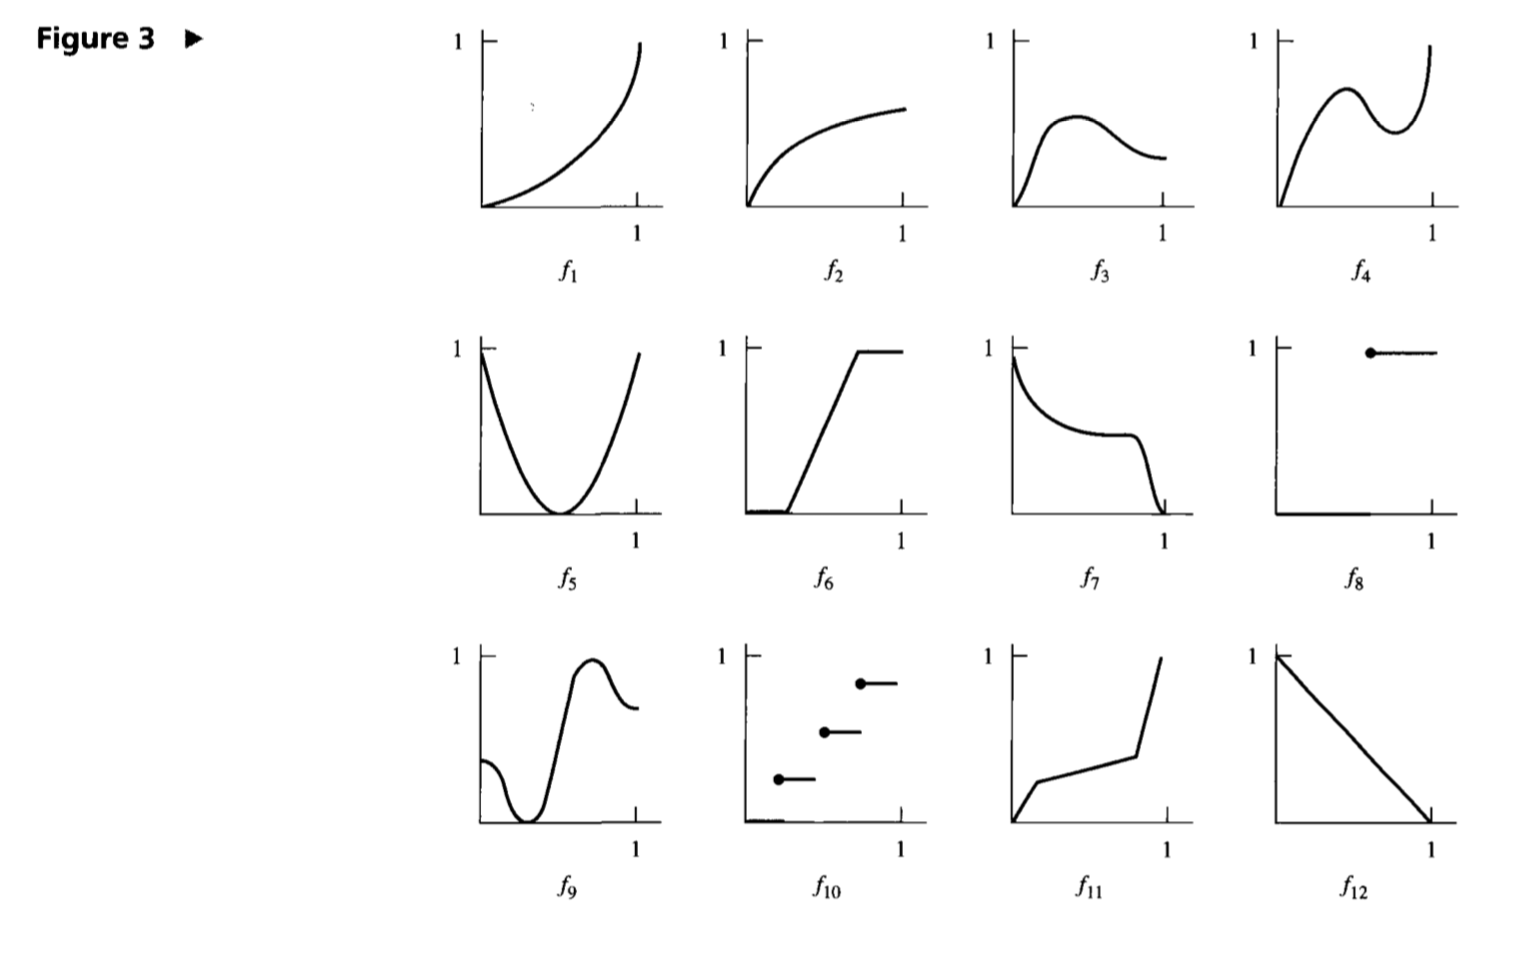
\includegraphics[width=\linewidth]{figure3.png}
\end{figure}
\textit{(TODO check with Professor about question 2)}
\end{center}

\subsection*{(a)}
\begin{center}
Which of these functions are one-to-one?\\
\hfill \break
$f_1, f_2, f_{11}$ because $x$ and $y$ coordinates are not repeated on $x$ and $y$ axes.
\end{center}

\hfill \break
\subsection*{(b)}
\begin{center}
Which of these functions map $[0,1]$ onto $[0,1]$?\\
\hfill \break
Might be a bit of a trick question; the original statement tells us that all functions have domain and codomain mapped to $[0,1]$.
\end{center}

\subsection*{(c)}
\begin{center}
Which of these functions are one-to-one correspondences?\\
\hfill \break
$f_{12}$ because the graph is symmetrical diagonally with no repeated points on $x$ and $y$ axes.
\end{center}
%
%
\subsection*{3.}
\begin{center}
The function $f(m,n) = 2^{m}3^{n}$ is a one-to-one function from $\mathbb{N} \times \mathbb{N} \text{ into } \mathbb{N}$.
\end{center}

\subsection*{(a)}
\begin{center}
Calculate $f(m,n)$ for five different elements $(m,n)$ in $\mathbb{N} \times \mathbb{N}$:\\
\hfill \break
$f(0,1) = 2^{0}3^{1} = 1 \cdot 3 = 3$\\
$f(2,3) = 2^{2}3^{3} = 4 \cdot 27 = 108$\\
$f(1,2) = 2^{1}3^{2} = 2 \cdot 9 = 18$\\
$f(0,2) = 2^{0}3^{2} = 1 \cdot 9 = 9$\\
$f(0,3) = 2^{0}3^{3} = 1 \cdot 27 = 27$ 
\end{center}
%
%
\subsection*{4.}
\begin{center}
Consider the following functions from $\mathbb{N} \text{ into } \mathbb{N}$:\\
$1_{\mathbb{N}}(n) = n, f(n) = 3n, g(n) = n + (-1)^{n}, h(n) = \text{min}[n, 100], k(n) = \text{max}[0, n - 5]$
\end{center}

\subsection*{(a)}
\begin{center}
Which of these functions are one-to-one?\\
\hfill \break
$1_{\mathbb{N}}(n)$\\
$f(n)$\\
$g(n)$
\end{center}

\subsection*{(b)}
\begin{center}
Which of these functions map $\mathbb{N} \text{ into } \mathbb{N}$?\\
\hfill \break
these cover all values in the $\mathbb{N}$ codomain:\\
$1_{\mathbb{N}}(n)$\\
$g(n)$
\end{center}
%
%
\subsection*{5.}
\begin{center}

\end{center}

\subsection*{(a)}
\begin{center}

\hfill \break

\end{center}

\subsection*{(b)}
\begin{center}

\hfill \break

\end{center}

\subsection*{(c)}
\begin{center}

\hfill \break

\end{center}

\subsection*{(d)}
\begin{center}

\hfill \break

\end{center}

\subsection*{(e)}
\begin{center}

\hfill \break

\end{center}
%
%



\end{document}
